\documentclass [12pt, a4paper] {article}

\usepackage[all, knot] {xy}
\let\oldxy\xy\def\xy{\begingroup\catcode`\"12\oldxy}
\let\oldendxy\endxy\def\endxy{\oldendxy\endgroup} 
\xyoption {arc}
\usepackage [latin1] {inputenc}
\usepackage [T1] {fontenc}
\usepackage [english] {babel}
\usepackage [dvips] {graphicx}
\usepackage {amsfonts}
\usepackage {amssymb}
\usepackage {amsmath}
\usepackage {verbatim}
\usepackage {fancyhdr}
\usepackage {psfrag}
\usepackage {listings}
\usepackage {eso-pic}
\usepackage {wasysym}
\usepackage {longtable}

%\usepackage[urw-garamond]{mathdesign}
\usepackage[small,bf]{caption}

\addtolength{\evensidemargin}{-1cm}
\addtolength{\oddsidemargin}{-1cm}
\addtolength{\marginparwidth}{-2.0cm}
\addtolength{\topmargin}{-2cm}
\addtolength{\textwidth}{3cm}
\addtolength{\textheight}{2cm}
\addtolength{\columnsep}{0.5cm}

 
\lhead {Coordinate Systems for Satellites\\ Derivations }
\rhead {Ville R\"{a}is\"{a}nen \\ \today}
\thispagestyle{fancy}

\newtheorem {teht} {Teht�v�} 
\newtheorem {maar} {M��ritelm�} 
\newtheorem {lemma} {Lemma} 
\newtheorem {lause} {Theorem} 
\newtheorem {kysymys} {Kysymys} 
\newtheorem {havainto} {Havainto} 
\newtheorem {seuraus} {Seuraus}
\newtheorem {oletus} {Oletus}
\newcommand{\sind}
{
	\textrm{sind}
}
\newcommand{\cosd}
{
	\textrm{cosd}
}
\newcommand{\vu}[1]
{
	\mathbf{\hat #1}
}
\newcommand{\vf}[1]
{
	\mathbf{\vec #1}
}
\newcommand{\mc}[1]
{
	\mathcal{#1}
}
\newcommand{\vc}[1]
{
	\boldsymbol{#1}
}
\newcommand{\vcc}[1]
{
	\widetilde{\boldsymbol{#1}}
}
\newcommand{\cc}[1]
{
	\widetilde{#1}
}
\newcommand{\sgn}
{
  \textrm{sgn}\:
}
\newcommand{\pdiff}[2]
{
	\frac{\partial #1}{\partial #2}
}
\newcommand{\diff}[2]
{
	\frac{d #1}{d #2}
}
\newcommand{\vali}
{
  \begin {displaymath}\:\end{displaymath}
}
\newcommand{\norm}[2]
{
  ||#1||_{#2}
}
\begin {document}
\begin {figure}
  \begin {center}
     \psfrag{NEP}[][l][2]{NEP}
     \psfrag{NCP1}[][t][2]{NCP(2000 AD)}
     \psfrag{NCP2}[][t][2]{NCP(11000 BC)}
     \psfrag{Polaris}[][lb][2]{Polaris}

     \psfrag{AE}[][lb][2.5]{$-\aries$}
     \psfrag{VE}[][lb][2.5]{$\aries$}
     \psfrag{Eqplane}[][lb][2.5]{Equatorial}
     \psfrag{Ecplane}[][lb][2.5]{Ecliptic}
     \psfrag{Sun}[][lb][4.5]{$\sun$}
     \psfrag{Earth}[][lb][4.5]{$\earth$}
     \psfrag{angle}[][lb][2.5]{$23.5^\circ$}

     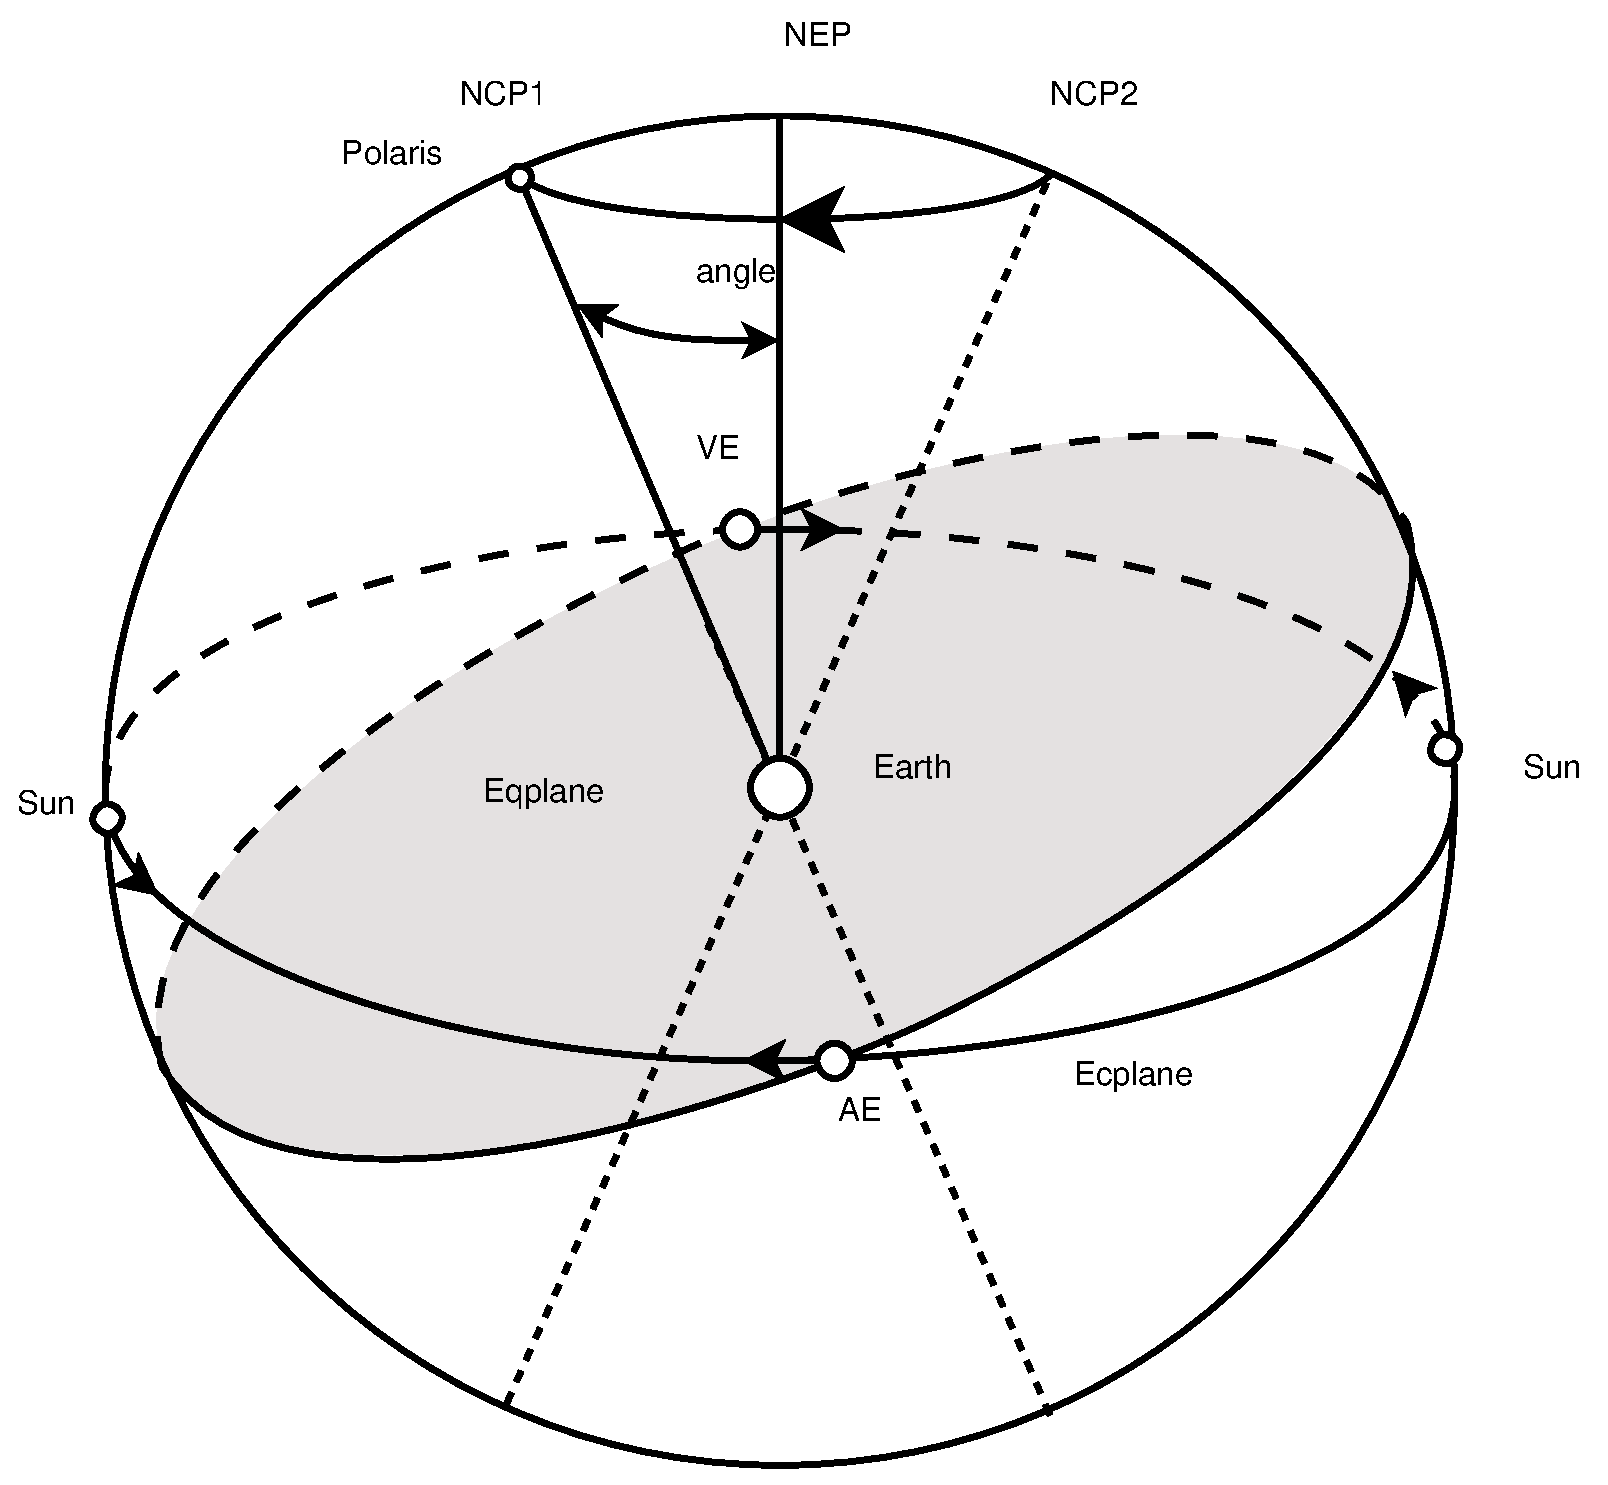
\includegraphics [angle=0, width=0.6\columnwidth] {figures/precession.eps}
     \caption{\label{fig:planes}Movement of the Vernal Equinox $\aries$ at the intersection of 
     Equatorial and Ecliptic Planes due to precession and its influence on the rotation 
     of Northern Celestial Pole (NCP) around the Northern Ecliptic Pole (NEP).}
  \end {center}
\end {figure} 
The \emph{ecliptic plane} is the plane that contains the orbit of the Earth $(\earth)$ around
the Sun $(\sun)$. The \emph{equatorial plane} of the Earth defines its axis of rotation. The axis is 
influenced by
\begin {enumerate}
  \item Precession with a 25772 year period. 
  \item Nutation with 18.6 year period with an amplitude of 9.2 arcseconds. 
  \item Polar motion with two components having 14- and 12-month periods.
\end {enumerate}
The \emph{mean equatorial plane} includes the effect of precession but the effect of nutation
is averaged out. The \emph{true equatorial plane} includes both the effects of precession 
and nutation.

The intersection of the ecliptic and equatorial planes is called the \emph{vernal equinox}
($\aries$, see Figure \ref{fig:planes}).
Since there are two directions associated to the intersection, the vernal equinox as a 
direction refers to the direction, where in March when the Sun travels through this intersection
to the side of northern hemisphere.
The \emph{mean and true vernal equinoxes} are the intersections of the ecliptic plane with 
the mean and true equatorial planes, respectively.

The mean vernal equinox at the \emph{J2000.0 epoch} is an important reference direction.
The J2000.0 epoch is precisely Julian date 2451545.0 TT (Terrestial Time) or January 1, 2000
noon TT. This is equivalent to January 1, 2000 11:59:27.816 TAI or January 1, 2000
11:58:55.816 UTC.


\section{Time Conversions}
Accurate computation of positions and orientations in space requires availability of 
conversions between different time standards. Personal computers can be synchronized 
over the Internet to UTC time with an accuracy of tens of milliseconds but availability 
of UTC time even with perfect availability does not alone allow accurate computations:
The orientation of the Earth is coupled to UT1 time, which may differ from UTC time as 
much as $0.9$ seconds.
Satellite instruments often rely on atomic TAI time, which is decoupled from variations
in the rotation of the Earth.

In amateur astronomy, an error of one second can be usually ignored but an error of
one second can correspond to an error of $8$ kilometers in the position of a satellite
on low Earth orbit (LEO).

\subsection{Time Standards}
\subsubsection{Solar Time}
\emph{Apparent (or true) solar time} is based on the movement of the Sun across the sky.
A \emph{solar day} is the time between two transits of the Sun over a local meridian. The
length of a solar day is dependent on the location of the Earth on its slightly elliptic
orbit. \emph{Mean solar time} tracks theoretical mean movement of the Sun with uniform 
movement across the celestial equator. Watches keep track of mean solar time while sundials
measure the apparent solar time. The relationship between the two is called the 
\emph{equation of time}.

\subsubsection{Sidereal Time}
Apparent solar time contains contributions from both the rotation of the Earth and the
movement of the Earth around Sun. The component related to the rotation is called 
\emph{sidereal time}. \emph{Sidereal day} is approximately $86164.0905\:$s while mean solar
day is approximately $86400.002\:$s. 

There are four varieties of sidereal time (see Figure \ref{fig:sidereal}): 
\begin {itemize}
  \item \emph{Greenwich Apparent Sidereal Time} (GAST) is the clockwise angle from the meridian 
  of the true vernal equinox to the Greenwich zero meridian.
  \item \emph{Greenwich Mean Sidereal Time} (GMST) is the clockwise angle from the meridian 
  of the mean vernal equinox to the Greenwich zero meridian.
  \item \emph{Local Apparent Sidereal Time} (LAST) is the clockwise angle from the meridian of 
  the true vernal equinox to the local meridian.
  \item \emph{Local Mean Sidereal Time} (LMST) is the clockwise angle from the meridian of the 
  mean vernal equinox to the local meridian. 
\end {itemize}
\begin {figure}
  \begin {center}
    \psfrag{Equator}[][][2]{Equatorial Plane}
    \psfrag{tvernal}[][][2]{$\aries$ (True)}
    \psfrag{mvernal}[][][2]{$\aries$ (Mean)}
    \psfrag{GAST}[][r][2]{GAST}
    \psfrag{GMST}[][r][2]{GMST}
    \psfrag{LAST}[][][2]{$\:\:$LAST}
    \psfrag{LMST}[][r][2]{LMST}
    \psfrag{greenwich}[][][2]{Greenwich}
 
     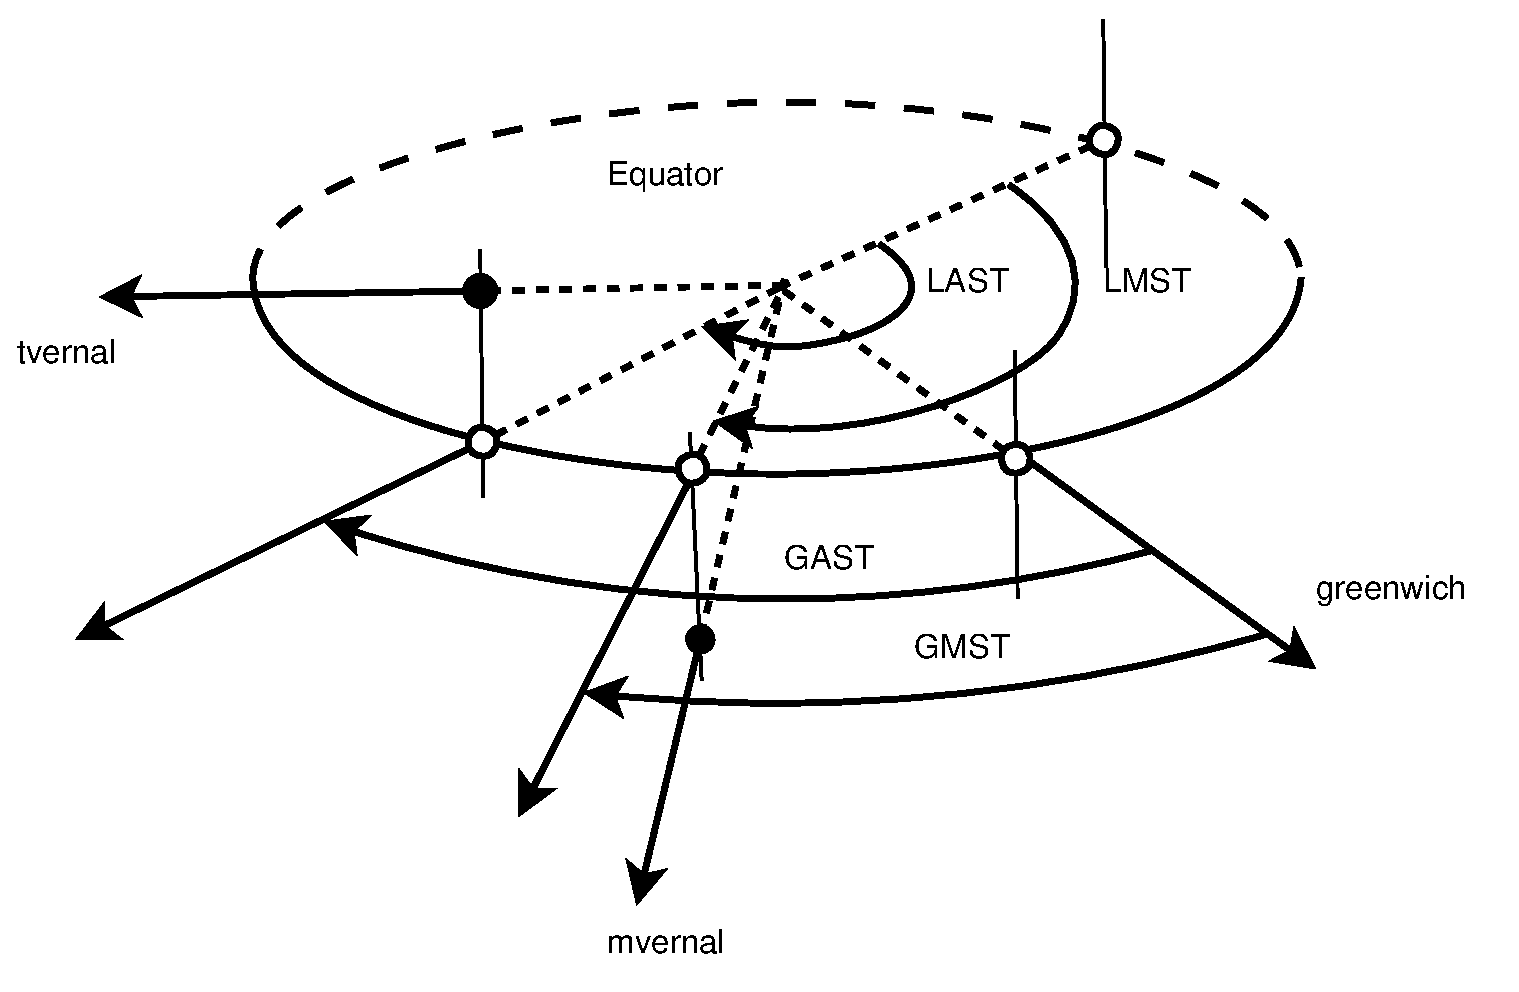
\includegraphics [angle=0, width=0.75\columnwidth] {figures/GAST.eps}
     \caption{\label{fig:sidereal}Types of sidereal time. Vertical lines correspond 
     to meridians. The angle between true and mean vernal equinox is exaggerated.}
  \end {center}
\end {figure} 
The mean and apparent varieties are related by the \emph{equation of the equinoxes}:
\begin {eqnarray}
  \label{eq:equinoxes}
  \textrm{GMST} - \textrm{GAST} = \textrm{LMST} - \textrm{LAST} = \alpha_E,
\end {eqnarray}
where $\alpha_E$ is a nutational parameter (\ref{eq:nutpar}). Greenwich and local 
varieties are related by 
\begin {eqnarray}
  \textrm{LMST} - \textrm{GMST} = \textrm{LAST} - \textrm{GAST} = \lambda
\end {eqnarray}
where $\lambda$ is the east longitude of the local meridian.

\subsubsection{Universal Time}
The \emph{UT1 time} describes roughly the rotation angle of the Earth scaled by the factor
\begin {eqnarray}
  \textrm{one mean Solar day} / \textrm{one sidereal day}.
\end {eqnarray}
with additional adjustments for polar motion. It is defined via the relationship:
\begin {eqnarray}
\label{eq:gmst}
\textrm{GMST} &=& 1.002\,737\,909\,350\,795\cdot\textrm{UT1} + \textrm{GMST}_0,
\end {eqnarray}
where UT1$\in[0.0\:\textrm{h}, 24.0\:\textrm{h})$ and Greenwich Mean Sidereal Time at 
$0^h$ UT1:
\begin {eqnarray}
  \label{eq:gmst_0}
  \textrm{GMST}_0 := 6^h41^m50^s.548\,51 + 8\,640\,184^s.812\,866\:T_u + 
  0^s.093\,104\:T_u^2 - 6^s.2\,10^{-6}T_u^3,
\end {eqnarray}
and 
\begin {eqnarray}
  T_u &:=& \dfrac{JD - 2\,451\,545}{36\,525}.
\end {eqnarray}
The Julian Date in the above is w.r.t. UT1 and points to the UT1 midnight of the day. 
Thus, it has the fractional part $.5$.
The linear term in $(\ref{eq:gmst_0})$ corresponds to the orbit of the Earth around the 
Sun and corresponds to the fractional part in $(\ref{eq:gmst})$:
\begin {eqnarray}
  8\,640\,184^s.812\,866 \:\frac{\Delta JD}{36\,525} 
  = 0^h.002\,737\,909\,350\,795\cdot 24\:\Delta JD.
\end {eqnarray}

%\lstset{basicstyle=\footnotesize\ttfamily, breaklines=true}
%\lstinputlisting[language=Matlab] {matlab/sidereal_time_gmst.m}


\subsubsection{Atomic Time and Coordinated Universal Time}
\emph{International Atomic Time} (TAI) is based on notional passage of proper time on 
Earth's geoid. Passage of TAI is continuous based on weighted average of 400 
atomic clocks worldwide. TAI forms the basis \emph{Coordinated Universal Time} (UTC),
which deviates from TAI by integer number of leap seconds. Leap seconds are introduced
at 
\begin {displaymath}
  \textrm{December 31  23:59:60} \:\textrm{UTC}
\end {displaymath}
of suitable years so that 
\begin {eqnarray}
  |\textrm{UTC} - \textrm{UT1}| < 0.9\:\textrm{s}
\end {eqnarray}
holds at every given moment in time.

\subsection{Earth Orientation Parameters}
Since the rotation of the Earth determines UT1 and the rotation cannot be 
accurately predicted, the relationship between UT1, TAI and UTC has to be 
obtained from measurement of the rotation of the Earth. 

The U.S. Naval Observatory's Earth Orientation Department is responsible for
determining and predicting Earth Orientation Parameters (EOPs), which describes
the time-varying orientation of the Earth. The EOPs are determined from radio 
telescope measurements of objects billions of light years away. The EOPs are 
part of the bulletins published by the International Earth Rotation and Reference
Systems Service (IERS). IERS Bulletin A includes predictions for: 
\begin {itemize}
  \item TAI - UTC difference,
  \item UT1 - UTC (DUT1) difference,
  \item Polar motion parameters $x$ and $y$
\end {itemize}
as well as measured errors for past predictions.


\newpage
\section{Reference Systems and Frames}
A conventional \emph{coordinate or reference system} is a set of prescriptions that defines 
a triad of orthogonal axes at any time whereas conventional \emph{frame} is the practical 
realization of a system at a specific epoch based on the system prescriptions. Reference 
frames and their relationships discussed in this section are depicted in 
Figure $\ref{fig:coordinates}$.

The discussion of Earth-Centered Frames is based on \cite{gnss} and \cite{aiaa_frames}.
\begin {figure}
  \begin {center}
     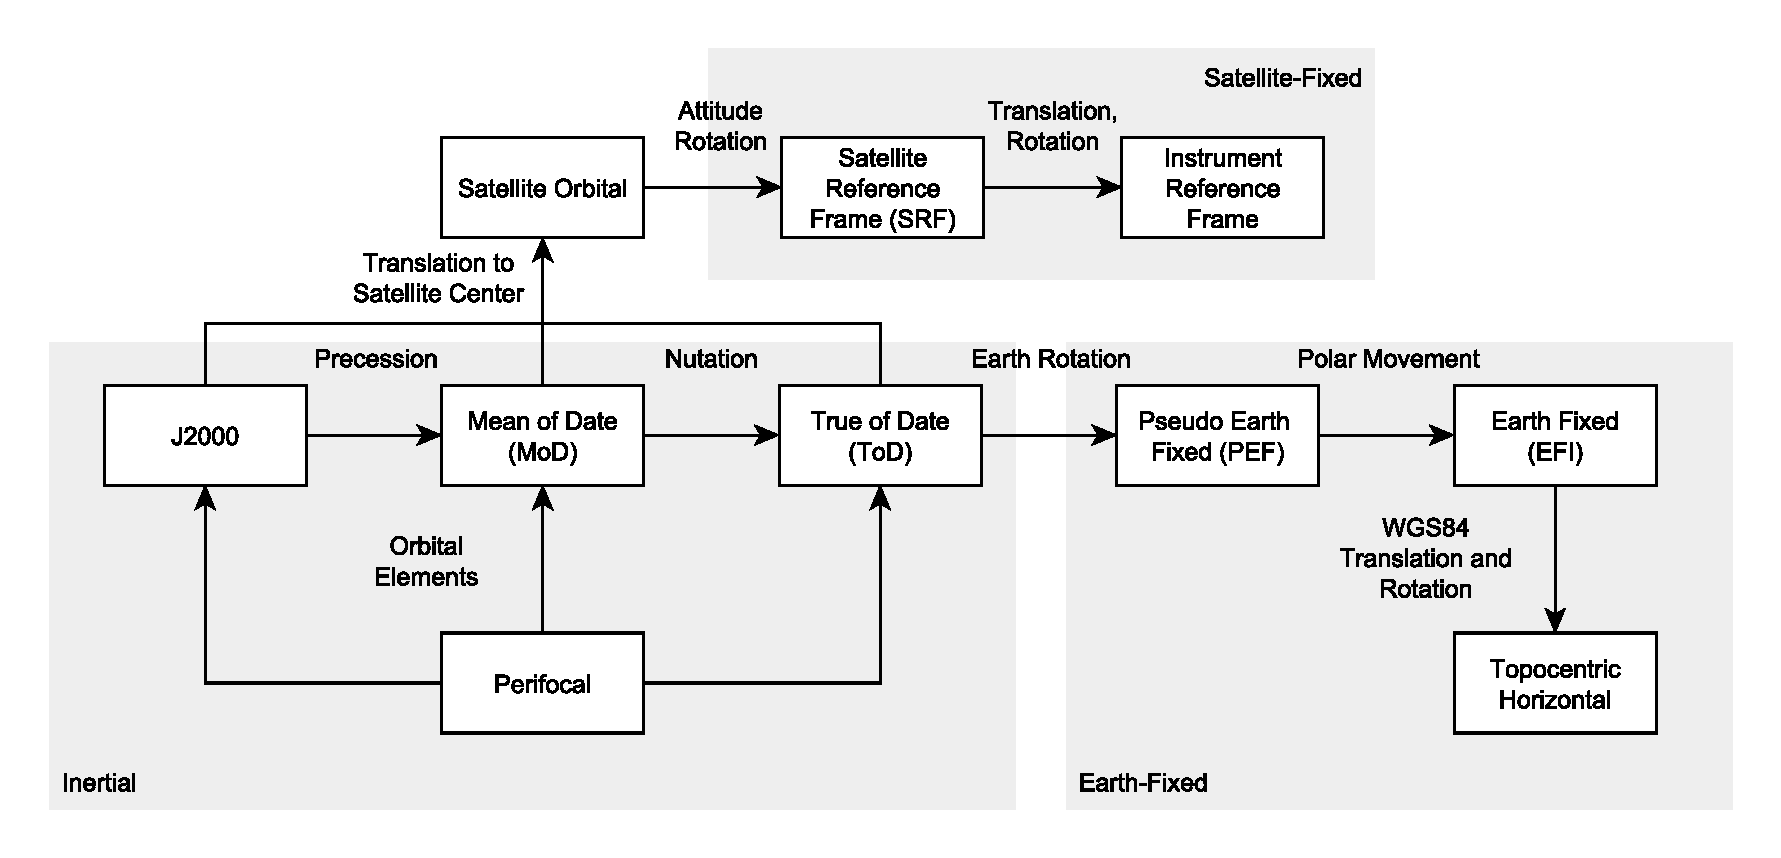
\includegraphics [angle=0, width=1.0\columnwidth] {figures/coordinates.eps}
     \caption{\label{fig:coordinates} Frames related to satellite orbits and transformation between 
     them.}
  \end {center}
\end {figure} 


\subsection{Earth-Centered Systems}
Earth-Centered Systems have their origin in the barycenter (also called geocenter) of
the Earth. Such systems are also called \emph{geocentric} \cite{gnss}.
Geocentric systems are related to each other by only rotations. 
In general, a RHS system is used, where the Z-axis matches the axis of rotation and in 
inertial systems, the X-axis points towards the vernal equinox.

\subsubsection{J2000 System}
The mean equator and equinox J2000.0 were defined by the International Astronomical Union 
(IAU) agreements in 1976 with 1980 nutation series \cite{GNSS}. Definitions
\begin {itemize}
  \item The X-axis points in the direction of the (computed?) mean vernal equinox at the 
  J2000.0 epoch.
  \item The Y-axis is orthogonal to X and Z axes to produce a RHS system.
  \item The Z-axis is orthogonal to the plane defined by the mean equator at the 
  J2000.0 epoch.
\end {itemize}
lead to a reference system called 
\emph{Conventional Celestial Reference System (CRS)}
also called the \emph{J2000 system} or \emph{GM2000 system}. 

\subsubsection{Mean of Date Reference System}
The \emph{Mean of Date (MoD) Reference System} is identical to the J2000.0/GM2000 system except
that the equatorial plane is determined according to current (of date) mean vernal equinox
and mean equatorial plane. That is, 
\begin {itemize}
  \item The X-axis points in the direction of the of date mean vernal equinox.
  \item The Y-axis is orthogonal to X and Z axes to produce a RHS system.
  \item The Z-axis is orthogonal to the plane defined by the of date mean equator.
\end {itemize}

\subsubsection{True of Date Reference System}
The \emph{True of Date (ToD) Reference System} is identical to the J2000.0/GM2000 frame except
that the equatorial plane is determined according to current (of date) true vernal equinox
and true equatorial plane. That is, 
\begin {itemize}
  \item The X-axis points in the direction of the of date true vernal equinox.
  \item The Y-axis is orthogonal to X and Z axes to produce a RHS system.
  \item The Z-axis is orthogonal to the plane defined by the of date true equator.
\end {itemize}

\subsubsection{Earth Fixed System}
The \emph{Earth Fixed System (EFI)} is the \emph{IERS Terrestial Reference System}, which is 
compatible with the WGS 84:
\begin {itemize}
  \item The X-axis is the intersection of the IERS Reference Meridian (IRM) 
  and the plane passing through the origin and normal to the Z-axis. 
  \item The Y-axis is orthogonal to X and Z axes to produce a RHS system.
  \item The Z-axis points to the direction IERS Reference Pole (IRP).
\end {itemize}
The IRM is the prime meridian with $0^\circ$ longitude maintained by the IERS. 

\subsubsection{Pseudo Earth Fixed System}
The \emph{Pseudo Earth Fixed (PEF) System} is equal to the Earth Fixed System without polar motion.
The system is also called the \emph{Earth Centered Earth Fixed (ECEF)} system.

\subsection{Conversions Between Earth-Centered Frames}
The rotation matrices between the Earth-centered frames are as follows,
\begin {eqnarray}
  \textrm{J2000}
  \overset{P}{\mapsto}
  \textrm{MoD}
  \overset{N}{\mapsto}
  \textrm{ToD}
  \overset{R}{\mapsto}
  \textrm{PEF}
  \overset{R_M}{\mapsto}
  \textrm{EFI}
\end {eqnarray}
where the rotation matrices are defined as follows:
\begin {eqnarray}
  P &=& R_z(-z)R_y(\nu)R_z(-\zeta) \\
  N &=& R_x(-\epsilon')R_z(-\Delta\psi)R_x(\epsilon) \\
  R &=& R_z(\textrm{GAST}) \\
  R_M &=& R_y(-x_p) R_x(-y_p),
\end {eqnarray}
where the rotation matrix parameters are defined in sections below. The rotation matrices
are defined as follows:
\begin {eqnarray}
  R_x(\theta) := 
  \begin {bmatrix}
    1 & 0 & 0 \\
    0 & \cos\theta & \sin\theta \\
    0 & -\sin\theta & \cos\theta 
  \end {bmatrix}
  ,
  R_y(\theta) := 
  \begin {bmatrix}
    \cos\theta & 0 & - \sin\theta \\
    0 & 1 & 0 \\
    \sin\theta & 0 & \cos\theta 
  \end {bmatrix}
  ,
  R_z(\theta) := 
  \begin {bmatrix}
    \cos\theta & \sin\theta & 0 \\
    -\sin\theta & \cos\theta & 0 \\
    0 & 0 & 1
  \end {bmatrix}.
\end {eqnarray}
\subsubsection{Conversion Between J2000 to MoD Frames}
The conversion between J2000 and MoD frames is determined by the Precession matrix
\begin {eqnarray}
  P &=& R_z(-z)R_y(\nu)R_z(-\zeta),
\end {eqnarray}
where the angles are given by the expressions (IAU 1976 Precession Model):
\begin {eqnarray}
  \label{eq:precparam}
  z     &=& 2306''.2181\:T + 1''.094\,68\:T^2 + 0''.0182\,03\:T^3 \\\nonumber
  \nu   &=& 2004''.3109\:T - 0''.426\,65\:T^2 - 0''.0418\,33\:T^3 \\\nonumber
  \zeta &=& 2306''.2181\:T + 0''.301\,88\:T^2 + 0''.0179\,98\:T^3,
\end {eqnarray}
where
\begin {eqnarray}
  T= \frac{JT - 2\,451\,544.9992572}{36525.0} \approx 
  \frac{JT - 2\,451\,545}{36525.0}
\end {eqnarray} 
is the number of Julian centuries from the J2000.0 epoch.
$(\ref{eq:precparam})$ can be written in term of degrees
\begin {eqnarray}
  \begin {bmatrix}
    z\\\nu\\\zeta
  \end {bmatrix}
  =
  \begin {bmatrix}
    6.406161389^\circ\cdot 10^{-1} &  3.040777777^\circ\cdot 10^{-4} &  5.056388889^\circ\cdot 10^{-6} \\
    5.567530278^\circ\cdot 10^{-1} & -1.185138889^\circ\cdot 10^{-4} & -1.162027778^\circ\cdot 10^{-5} \\
    6.406161389^\circ\cdot 10^{-1} &  8.385555556^\circ\cdot 10^{-5} &  4.999444444^\circ\cdot 10^{-6}
  \end {bmatrix}
  \begin {bmatrix}
    T \\ T^2 \\ T^3
  \end {bmatrix}.
\end {eqnarray}

\subsubsection{Conversion Between MoD to ToD Frames}
The conversion between the MoD and ToD is determined by the Nutation matrix 
\begin {eqnarray}
  N &=& R_x(-\epsilon')R_z(-\Delta\psi)R_x(\epsilon),
\end {eqnarray}
where 
\begin {eqnarray}
  \epsilon' &=& \epsilon + \Delta\epsilon, \\
  \epsilon &=& 23^\circ 26'21''.448 - 46''.8150\:T - 0''.000\,59\:T^2 + 0''.001\,813T^3
  \\
  \nonumber &=& 
  23.4392911111^\circ - 0.0130041667^\circ\:T - 1.6388888889^\circ 10^{-7}\:T^2 
  + 5.0361111111^\circ\cdot 10^{-7}\:T^3,
  \\
  \Delta\psi &=& (10^{-4}\,'') \cdot
  \sum_{j=1}^N 
  \left[
    \left(A_{0j} + A_{1j}T\right)\sin\left(\sum_{i=1}^5 k_{ji}\alpha_i\right)
  \right], 
  \\
  \Delta\epsilon &=& (10^{-4}\,'') \cdot
  \sum_{j=1}^N 
  \left[
    \left(B_{0j} + B_{1j}T\right)\cos\left(\sum_{i=1}^5 k_{ji}\alpha_i\right)
  \right].
\end {eqnarray}
The parameters $\alpha_i$ are functions $T$:
Mean anomaly of the Moon 
\begin {eqnarray}
  \alpha_1 &=& 134.9629813889^\circ + 198.8673980555^\circ\:T + 8.6972222222^\circ\cdot 10^{-3}\:T^2 
   \\\nonumber &+& (1.7777777778^\circ\cdot 10^{-5}\:T^3) 
        + (1325.0 \cdot 360.0^\circ T).
\end {eqnarray}
Mean anomaly of the Sun
\begin {eqnarray}
  \alpha_2 &=& 357.5277233333^\circ + 359.0503400000^\circ\:T - 1.6027777778^\circ\cdot 10^{-4}\:T^2 
   \\\nonumber &-& (3.3333333333^\circ\cdot 10^{-6}\:T^3) 
        + (99.0 \cdot 360.0^\circ T).
\end {eqnarray}
Moon's mean argument of latitude
\begin {eqnarray}        
  \alpha_3 &=&  93.2719102778^\circ + 82.0175380556^\circ\:T   - 3.6825000000^\circ\cdot 10^{-3}\:T^2 
  \\\nonumber &+& (3.0555555555^\circ\cdot 10^{-6}\:T^3)
        + (1342.0 \cdot 360.0^\circ T).
\end {eqnarray}
Moon's mean elongation from the Sun
\begin {eqnarray}        
  \alpha_4 &=& 297.8503630555^\circ + 307.1114800000^\circ\:T  - 1.9141666667^\circ\cdot 10^{-3}\:T^2 
  \\\nonumber &+& (5.2777777778^\circ\cdot 10^{-6}\:T^3)
        + (1236.0 \cdot 360.0^\circ T).
\end {eqnarray}
Mean longitude of the ascending lunar node
\begin {eqnarray}
  \alpha_5 &=& 125.0445222222^\circ - 134.1362608333^\circ\:T + 2.0708333333^\circ\cdot 10^{-3}\:T^2
  \\\nonumber &+& (2.2222222222^\circ\cdot 10^{-6}\:T^3)
        - (5.0 \cdot 360.0^\circ T).
\end {eqnarray}
The parameters $A_{0j}, A_{1j}, B_{0j}, B_{1j}$ are listed in Table \ref{table:nutcoeff}. 
\begin {center}
  \begin {longtable}{| c | c c c c c | c | c | c | c | r |}
    \hline 
    $i$ & $k_{i1}$ & $k_{i2}$ & $k_{i3}$ & $k_{i4}$ &  $k_{i5}$ & Period & $A_{0j}$ & $A_{1j}$ & $B_{0j}$  & $B_{1j}$ \\
    \hline
    \endhead
      1 & 0&   0&   0&   0&   1&   -6798.4& -171996.0&    -174.2&   92025.0&       8.9 \\
      2 & 0&   0&   2&  -2&   2&     182.6&  -13187.0&      -1.6&    5736.0&      -3.1 \\
      3 & 0&   0&   2&   0&   2&      13.7&   -2274.0&      -0.2&     977.0&      -0.5 \\
      4 & 0&   0&   0&   0&   2&   -3399.2&    2062.0&       0.2&    -895.0&       0.5 \\
      5 & 0&  -1&   0&   0&   0&    -365.3&   -1426.0&       3.4&      54.0&      -0.1 \\
      6 & 1&   0&   0&   0&   0&      27.6&     712.0&       0.1&      -7.0&       0.0 \\
      7 & 0&   1&   2&  -2&   2&     121.7&    -517.0&       1.2&     224.0&      -0.6 \\
      8 & 0&   0&   2&   0&   1&      13.6&    -386.0&      -0.4&     200.0&       0.0 \\
      9 & 1&   0&   2&   0&   2&       9.1&    -301.0&       0.0&     129.0&      -0.1 \\
      10 & 0&  -1&   2&  -2&   2&     365.2&     217.0&      -0.5&     -95.0&       0.3 \\
      11 & -1&   0&   0&   2&   0&      31.8&     158.0&       0.0&      -1.0&       0.0 \\
      12 & 0&   0&   2&  -2&   1&     177.8&     129.0&       0.1&     -70.0&       0.0 \\
      13 & -1&   0&   2&   0&   2&      27.1&     123.0&       0.0&     -53.0&       0.0 \\
      14 & 1&   0&   0&   0&   1&      27.7&      63.0&       0.1&     -33.0&       0.0 \\
      15 & 0&   0&   0&   2&   0&      14.8&      63.0&       0.0&      -2.0&       0.0 \\
      16 & -1&   0&   2&   2&   2&       9.6&     -59.0&       0.0&      26.0&       0.0 \\
      17 & -1&   0&   0&   0&   1&     -27.4&     -58.0&      -0.1&      32.0&       0.0 \\
      18 & 1&   0&   2&   0&   1&       9.1&     -51.0&       0.0&      27.0&       0.0 \\
      19 & -2&   0&   0&   2&   0&    -205.9&     -48.0&       0.0&       1.0&       0.0 \\
      20 & -2&   0&   2&   0&   1&    1305.5&      46.0&       0.0&     -24.0&       0.0 \\
      21 & 0&   0&   2&   2&   2&       7.1&     -38.0&       0.0&      16.0&       0.0 \\
      22 & 2&   0&   2&   0&   2&       6.9&     -31.0&       0.0&      13.0&       0.0 \\
      23 & 2&   0&   0&   0&   0&      13.8&      29.0&       0.0&      -1.0&       0.0 \\
      24 & 1&   0&   2&  -2&   2&      23.9&      29.0&       0.0&     -12.0&       0.0 \\
      25 & 0&   0&   2&   0&   0&      13.6&      26.0&       0.0&      -1.0&       0.0 \\
      26 & 0&   0&   2&  -2&   0&     173.3&     -22.0&       0.0&       0.0&       0.0 \\
      27 & -1&   0&   2&   0&   1&      27.0&      21.0&       0.0&     -10.0&       0.0 \\
      28 & 0&   2&   0&   0&   0&     182.6&      17.0&      -0.1&       0.0&       0.0 \\
      29 & 0&   2&   2&  -2&   2&      91.3&     -16.0&       0.1&       7.0&       0.0 \\
      30 & -1&   0&   0&   2&   1&      32.0&      16.0&       0.0&      -8.0&       0.0 \\
      31 & 0&   1&   0&   0&   1&     386.0&     -15.0&       0.0&       9.0&       0.0 \\
      32 & 1&   0&   0&  -2&   1&     -31.7&     -13.0&       0.0&       7.0&       0.0 \\
      33 & 0&  -1&   0&   0&   1&    -346.6&     -12.0&       0.0&       6.0&       0.0 \\
      34 & 2&   0&  -2&   0&   0&   -1095.2&      11.0&       0.0&       0.0&       0.0 \\
      35 & -1&   0&   2&   2&   1&       9.5&     -10.0&       0.0&       5.0&       0.0 \\
      36 & 1&   0&   2&   2&   2&       5.6&      -8.0&       0.0&       3.0&       0.0 \\
      37 & 0&  -1&   2&   0&   2&      14.2&      -7.0&       0.0&       3.0&       0.0 \\
      38 & 0&   0&   2&   2&   1&       7.1&      -7.0&       0.0&       3.0&       0.0 \\
      39 & 1&   1&   0&  -2&   0&     -34.8&      -7.0&       0.0&       0.0&       0.0 \\
      40 & 0&   1&   2&   0&   2&      13.2&       7.0&       0.0&      -3.0&       0.0 \\
      41 & -2&   0&   0&   2&   1&    -199.8&      -6.0&       0.0&       3.0&       0.0 \\
      42 & 0&   0&   0&   2&   1&      14.8&      -6.0&       0.0&       3.0&       0.0 \\
      43 & 2&   0&   2&  -2&   2&      12.8&       6.0&       0.0&      -3.0&       0.0 \\
      44 & 1&   0&   0&   2&   0&       9.6&       6.0&       0.0&       0.0&       0.0 \\
      45 & 1&   0&   2&  -2&   1&      23.9&       6.0&       0.0&      -3.0&       0.0 \\
      46 & 0&   0&   0&  -2&   1&     -14.7&      -5.0&       0.0&       3.0&       0.0 \\
      47 & 0&  -1&   2&  -2&   1&     346.6&      -5.0&       0.0&       3.0&       0.0 \\
      48 & 2&   0&   2&   0&   1&       6.9&      -5.0&       0.0&       3.0&       0.0 \\
      49 & 1&  -1&   0&   0&   0&      29.8&       5.0&       0.0&       0.0&       0.0 \\
      50 & 1&   0&   0&  -1&   0&     411.8&      -4.0&       0.0&       0.0&       0.0 \\
      51 & 0&   0&   0&   1&   0&      29.5&      -4.0&       0.0&       0.0&       0.0 \\
      52 & 0&   1&   0&  -2&   0&     -15.4&      -4.0&       0.0&       0.0&       0.0 \\
      53 & 1&   0&  -2&   0&   0&     -26.9&       4.0&       0.0&       0.0&       0.0 \\
      54 & 2&   0&   0&  -2&   1&     212.3&       4.0&       0.0&      -2.0&       0.0 \\
      55 & 0&   1&   2&  -2&   1&     119.6&       4.0&       0.0&      -2.0&       0.0 \\
      56 & 1&   1&   0&   0&   0&      25.6&      -3.0&       0.0&       0.0&       0.0 \\
      57 & 1&  -1&   0&  -1&   0&   -3232.9&      -3.0&       0.0&       0.0&       0.0 \\
      58 & -1&  -1&   2&   2&   2&       9.8&      -3.0&       0.0&       1.0&       0.0 \\
      59 & 0&  -1&   2&   2&   2&       7.2&      -3.0&       0.0&       1.0&       0.0 \\
      60 & 1&  -1&   2&   0&   2&       9.4&      -3.0&       0.0&       1.0&       0.0 \\
      61 & 3&   0&   2&   0&   2&       5.5&      -3.0&       0.0&       1.0&       0.0 \\
      62 & -2&   0&   2&   0&   2&    1615.7&      -3.0&       0.0&       1.0&       0.0 \\
      63 & 1&   0&   2&   0&   0&       9.1&       3.0&       0.0&       0.0&       0.0 \\
      64 & -1&   0&   2&   4&   2&       5.8&      -2.0&       0.0&       1.0&       0.0 \\
      65 & 1&   0&   0&   0&   2&      27.8&      -2.0&       0.0&       1.0&       0.0 \\
      66 & -1&   0&   2&  -2&   1&     -32.6&      -2.0&       0.0&       1.0&       0.0 \\
      67 & 0&  -2&   2&  -2&   1&    6786.3&      -2.0&       0.0&       1.0&       0.0 \\
      68 & -2&   0&   0&   0&   1&     -13.7&      -2.0&       0.0&       1.0&       0.0 \\
      69 & 2&   0&   0&   0&   1&      13.8&       2.0&       0.0&      -1.0&       0.0 \\
      70 & 3&   0&   0&   0&   0&       9.2&       2.0&       0.0&       0.0&       0.0 \\
      71 & 1&   1&   2&   0&   2&       8.9&       2.0&       0.0&      -1.0&       0.0 \\
      72 & 0&   0&   2&   1&   2&       9.3&       2.0&       0.0&      -1.0&       0.0 \\
      73 & 1&   0&   0&   2&   1&       9.6&      -1.0&       0.0&       0.0&       0.0 \\
      74 & 1&   0&   2&   2&   1&       5.6&      -1.0&       0.0&       1.0&       0.0 \\
      75 & 1&   1&   0&  -2&   1&     -34.7&      -1.0&       0.0&       0.0&       0.0 \\
      76 & 0&   1&   0&   2&   0&      14.2&      -1.0&       0.0&       0.0&       0.0 \\
      77 & 0&   1&   2&  -2&   0&     117.5&      -1.0&       0.0&       0.0&       0.0 \\
      78 & 0&   1&  -2&   2&   0&    -329.8&      -1.0&       0.0&       0.0&       0.0 \\
      79 & 1&   0&  -2&   2&   0&      23.8&      -1.0&       0.0&       0.0&       0.0 \\
      80 & 1&   0&  -2&  -2&   0&      -9.5&      -1.0&       0.0&       0.0&       0.0 \\
      81 & 1&   0&   2&  -2&   0&      32.8&      -1.0&       0.0&       0.0&       0.0 \\
      82 & 1&   0&   0&  -4&   0&     -10.1&      -1.0&       0.0&       0.0&       0.0 \\
      83 & 2&   0&   0&  -4&   0&     -15.9&      -1.0&       0.0&       0.0&       0.0 \\
      84 & 0&   0&   2&   4&   2&       4.8&      -1.0&       0.0&       0.0&       0.0 \\
      85 & 0&   0&   2&  -1&   2&      25.4&      -1.0&       0.0&       0.0&       0.0 \\
      86 & -2&   0&   2&   4&   2&       7.3&      -1.0&       0.0&       1.0&       0.0 \\
      87 & 2&   0&   2&   2&   2&       4.7&      -1.0&       0.0&       0.0&       0.0 \\
      88 & 0&  -1&   2&   0&   1&      14.2&      -1.0&       0.0&       0.0&       0.0 \\
      89 & 0&   0&  -2&   0&   1&     -13.6&      -1.0&       0.0&       0.0&       0.0 \\
      90 & 0&   0&   4&  -2&   2&      12.7&       1.0&       0.0&       0.0&       0.0 \\
      91 & 0&   1&   0&   0&   2&     409.2&       1.0&       0.0&       0.0&       0.0 \\
      92 & 1&   1&   2&  -2&   2&      22.5&       1.0&       0.0&      -1.0&       0.0 \\
      93 & 3&   0&   2&  -2&   2&       8.7&       1.0&       0.0&       0.0&       0.0 \\
      94 & -2&   0&   2&   2&   2&      14.6&       1.0&       0.0&      -1.0&       0.0 \\
      95 & -1&   0&   0&   0&   2&     -27.3&       1.0&       0.0&      -1.0&       0.0 \\
      96 & 0&   0&  -2&   2&   1&    -169.0&       1.0&       0.0&       0.0&       0.0 \\
      97 & 0&   1&   2&   0&   1&      13.1&       1.0&       0.0&       0.0&       0.0 \\
      98 & -1&   0&   4&   0&   2&       9.1&       1.0&       0.0&       0.0&       0.0 \\
      99 & 2&   1&   0&  -2&   0&     131.7&       1.0&       0.0&       0.0&       0.0 \\
      100 & 2&   0&   0&   2&   0&       7.1&       1.0&       0.0&       0.0&       0.0 \\
      101 & 2&   0&   2&  -2&   1&      12.8&       1.0&       0.0&      -1.0&       0.0 \\
      102 & 2&   0&  -2&   0&   1&    -943.2&       1.0&       0.0&       0.0&       0.0 \\
      103 & 1&  -1&   0&  -2&   0&     -29.3&       1.0&       0.0&       0.0&       0.0 \\
      104 & -1&   0&   0&   1&   1&    -388.3&       1.0&       0.0&       0.0&       0.0 \\
      105 & -1&  -1&   0&   2&   1&      35.0&       1.0&       0.0&       0.0&       0.0 \\
      106 & 0&   1&   0&   1&   0&      27.3&       1.0&       0.0&       0.0&       0.0 \\
  \hline
  \caption{Coefficients $A_{0j}$, $A_{1j}$, $B_{0j}$, $B_{1j}$ for IAU1980 nutation model.
  \label{table:nutcoeff}}
  \end {longtable}
\end {center}

\subsubsection{Conversion Between ToD to PEF Frames}
The conversion between the ToD and PEF is determined by the \emph{Earth Rotation Matrix}
\begin {eqnarray}
  R &=& R_z(\textrm{GAST}),
\end {eqnarray}
where $\textrm{GAST}$ is the Greenwich Apparent Sidereal Time obtained from 
$(\ref{eq:equinoxes})$
\begin {eqnarray}
  \textrm{GAST} &=& \textrm{GMST} - \alpha_E,
\end {eqnarray}
where
\begin {eqnarray}
  \label{eq:nutpar}
  \alpha_E &=& \tan^{-1}\left(
    \dfrac{N_{12}}{N_{11}}
  \right).
\end {eqnarray}
To obtain a different representation of GMST, let us combine $(\ref{eq:gmst})$ and 
$(\ref{eq:gmst_0})$:
\begin {eqnarray}
  GMST 
  &=& 
  GMST_0 + c\:\textrm{UT1} \\
  \nonumber
  &=&
  b_0 + b_1T_u + b_2T_u^2 + b_3T_u^3 + c\cdot\textrm{UT1}
\end {eqnarray}
Conversion of the constants into degrees yields
\begin {eqnarray}
  \nonumber
  b_0 &=& 100.460\,618\,375^\circ\\
  \nonumber
  b_1' &:=& b_1 / 36525.0 = 0.985\,647\,366^\circ %\\
 % \nonumber
 % b_2 &=& 1.062^\circ\cdot 10^{-8} \\
 % \nonumber
 %b_3 &=& -7.0727^\circ\cdot 10^{-13} \\
\end {eqnarray}
For the constant $c$, we can compute
\begin {eqnarray}
  c\cdot\textrm{UT1
  } &=& 360.9856473662862^\circ\cdot(JT - JD) \\
  \nonumber 
  &=&
  (360^\circ + b_1')(JT - JD) 
\end {eqnarray}
Substituting this back, yields 
\begin {eqnarray}
  \nonumber
  GMST &=& b_0 + b_1'(JD - JD_{2000}^{noon}) + (360^\circ + b_1')(JT - JD) 
  + b_2T_u^2 + b_3T_u^3,
\end {eqnarray}
where $JD_{2000}^{noon}=2\,451\,545$ corresponds to the Julian UT1 date at January 1, 2000 12:00:00.
The preceding midnight corresponds to a value $JD_{2000} = 2\,451\,544.5 = JD_{2000}^{noon} -0.5$.
Taking into account to modulo arithmetic of angles
\begin {eqnarray}
  %c\cdot\textrm{UT1} &=& 
  (360^\circ + b_1')(JT - JD)
  &=& \nonumber
  (360^\circ + b_1') (JT - JD_{2000}) + (360^\circ + b_1')(JD_{2000} - JD)\\
  &=^m& \nonumber
  (360^\circ + b_1') (JT - JD_{2000}) + b_1'(JD_{2000} - JD).
\end {eqnarray}
Thus, we obtain
\begin {eqnarray}
  \textrm{GMST} &=&
  b_0 + b_1'(JD - JD_{2000} - 0.5) + (360^\circ + b_1')(JT - JD_{2000}) + b_1'(JD_{2000} - JD)
  + ..
  \nonumber 
  \\ &=& 
  b_0 - \frac{b_1'}{2} + (360^\circ + b_1')(JT - JD_{2000}) + b_2T_u^2 + b_3T_u^3.
\end {eqnarray}
Substituting the values, yields 
\begin {eqnarray}
  \label{eq:GMST_expansion}
  \textrm{GMST}
  &\approx&
  100.460\,618\,375^\circ + 360.985\,647\,366^\circ(JT - JD_{2000})\\
   &+& 2.90788^\circ\cdot10^{-13} (JT - JD_{2000})^2 - 5.3016^\circ\cdot 10^{-22}(JT - JD_{2000})^3.
\end {eqnarray}
\subsubsection{Conversion Between PEF and EFI Frames}
The conversion between the PEF and EFI is determined by the \emph{Polar Motion Matrix}
\begin {eqnarray}
  R_M &=& R_y(-x_p)R_x(-y_p),
\end {eqnarray}
where $x_p$ and $y_p$ are angles that can be obtained from the IERS Bulletin A.
\subsubsection{Conversion of Velocities}
For Earth-centered frames, the coordinate transformations between frames are 
rotations. Thus, if the relationship between frames $1$ and $2$ can be written
\begin {eqnarray}
  \vc r^2 = R\vc r^1
\end {eqnarray}
the conversion between velocities can be expressed as 
\begin {eqnarray}
  \vc v^2 &=& R\vc v^1 + \diff{R}{t}\vc r^1.
\end {eqnarray}
For all such conversions except the ToD $\leftrightarrow$ PEF transformation, 
$dR/dt$ is in order of arcseconds per year and can be ignored. 
For ToD$\rightarrow$PEF transformation, 
\begin {eqnarray}
  \vc r_p &=& R_z(\textrm{GAST})\vc r_{t}
\end {eqnarray}
and 
\begin {eqnarray}
  \vc v_p &=& R_z(\textrm{GAST})\vc v_t 
  + \diff{R_z}{t}R_z(GAST)\diff{GAST}{t}\vc r_t.
\end {eqnarray}
The GAST can be expanded as using $(\ref{eq:GMST_expansion})$
\begin {eqnarray}
  \textrm{GAST} &=& \sum_{k=0}^3 \alpha_k(JT - JD_{2000})^k - \alpha_E.
\end {eqnarray}
Time-derivative of this be written as 
\begin {eqnarray}
  \diff{\textrm{GAST}}{t} &=& 
  \frac{1}{86400}\sum_{k=1}^3 k\alpha_k (JT - JD_{2000})^{k-1}.
\end {eqnarray}
Thereafter, denoting $\theta = \textrm{GAST}$, we obtain
\begin {eqnarray}
  \vc v_p =
  R_z(\textrm{GAST})\vc v_t
  +
  \frac{1}{86400}
  \frac{2\pi}{360}
    \sum_{k=1}^3 k\alpha_k (JT - JD_{2000})^{k-1} 
  \begin {bmatrix}
    -\sind(\theta) & \cosd(\theta) & 0 \\
    -\cosd(\theta) & -\sind(\theta) & 0 \\
    0 & 0 & 0
  \end {bmatrix}\vc r_t,
\end {eqnarray}
where 
$\alpha_1 = 360.985\,647\,366^\circ$
$\alpha_2 = 2.90788^\circ\cdot 10^{-13}$
$\alpha_3 = -5.3016^\circ\cdot 10^{-22}$.

\subsection{Topocentric Systems}
\emph{Topocentric systems} are centered on a fixed point on the surface of the Earth.
Most relevant topocentric systems are \emph{Local Tangent Plane} (LTP) coordinates, where 
the axes are fixed to the local tangent plane to form an RHS system. 
Depending 
on the required accuracy, a tangent plane, a sphere, a reference ellipsoid, geoid or a digital elevation 
model can be used to model the surface. 

\subsubsection{Surface Appoximations}
There is no unique definition for the surface of the Earth nor height of topographic features.
%since the surface can be influenced 
%by topographic variation, waves, ice, snow cover and buildings. 
To first approximation, the surface can be approximated as a sphere. However, the surface 
is flattened at the poles and bulges out the equator, which can be approximated by an ellipsoid. 
The World Geodetic System 1984 (WGS84) defines such an reference 
ellipsoid and also an associated geoid. Both are used reference surfaces, that is,  
\emph{geodetic datums} to measure the height of the surface variations. 

The geoid is an expression \emph{mean sea level} (MSL) in terms of spherical harmonics selected 
based on the Earth Gravitational Model 2008. MSL expresses the hypothetical time-averaged sea level, 
which would occur at a specific location of sea or when a canal was digged to specific location. 
Height w.r.t. MSL is called \emph{orthometric height}. 

Earth observation satellites typically use \emph{ellipsoid height} w.r.t. the \emph{WGS84 ellipsoid}:
\begin {eqnarray}
\textrm{Semi-major axis}(a) &=& 6\,378\,137.0\:\textrm{m} \\
\textrm{Semi-minor axis}(b) &=& 6\,356\,752.314\,245\textrm{m} \\
\textrm{Eccentricity}(e) &=& \sqrt{(a^2 - b^2)}/a = 0.081819190842965,
\end {eqnarray}
where the semi-major and semi-minor axes are associated to the equator and the poles, respectively.


\begin {figure}[h]
  \begin {center}
    \psfrag{phi}[][][3]{$\varphi$}
    \psfrag{l}[][b][3]{$\theta$}
    \psfrag{h}[][rb][3]{$h$}
    \psfrag{P}[][][3]{$P$}
 
     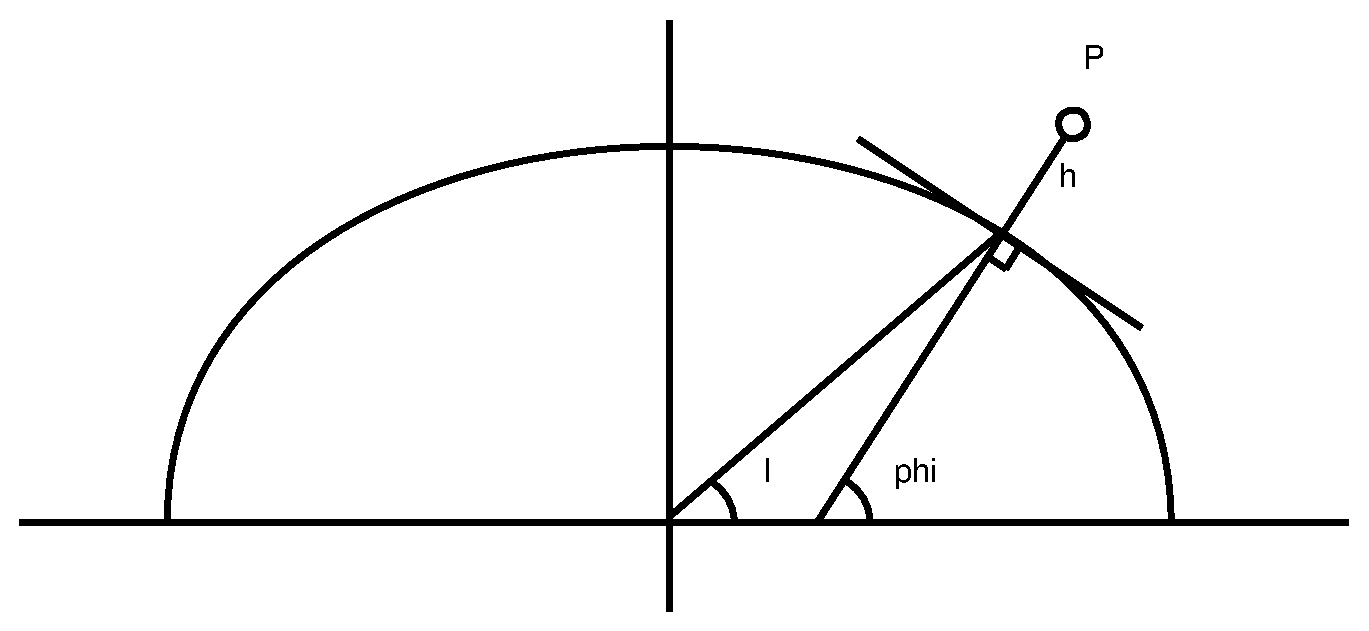
\includegraphics [angle=0, width=0.5\columnwidth] {figures/geodetic.eps}
     \caption{\label{fig:geodetic}Geocentric $\theta$ vs geodetic $\varphi$ latitude.}
  \end {center}
\end {figure} 
Cartesian coordinates in the EFI frame is related to the \emph{geodetic latitude} $\varphi$, 
\emph{geodetic longitude} $\lambda$ and \emph{height above the ellipsoid} as follows \cite{gnss}:
\begin {eqnarray}
  x &=& (N+h)\cos\varphi\cos\lambda \\
  y &=& (N+h)\cos\varphi\sin\lambda \\ 
  z &=& ((1-e^2)N + h) \sin\varphi,
\end {eqnarray}
where 
\begin {eqnarray}
   N &=& \frac{a}{\sqrt{1 - e^2\sin^2\varphi}}.
\end {eqnarray}
The longitude can be computed from the cartesian EFI coordinates with
\begin {eqnarray}
  \lambda &=& \textrm{atan2}(y, x).
\end {eqnarray}
For very distant objects such as stars, the angle between geocentric and geodetic latitude 
is small. When $h\gg a$ holds, we have $h \gg N$ and 
\begin {eqnarray}
  x &=& r\cos\varphi\cos\lambda \\
  y &=& r\cos\varphi\sin\lambda \\
  z &=& r\sin\varphi
\end {eqnarray}
where $r=h+a$. This allows solution 
\begin {eqnarray}
  \varphi = \arcsin\left(\frac{z}{h + a}\right)
\end {eqnarray}
For nearby objects, the latitude and height are obtained with the 
following iteration \cite{gnss}:
The initial value is given by: 
\begin {eqnarray}
  \varphi_{(0)} &=& \left(
    \dfrac{z/\sqrt{x^2 + y^2}}{1 - e^2}
  \right)
\end {eqnarray}
The iteration is given by:
\begin {eqnarray}
  N_{(i)} &=& \dfrac{a}{\sqrt{1 - e^2\sin^2\varphi_{(i-1)}}}, \\
  h_{(i)} &=& \dfrac{p}{\cos\varphi_{(i-1))}} - N_{(i)}, \\
  \varphi_{(i)} &=& \textrm{arctan}\left[
    \dfrac{z/\sqrt{x^2 + y^2}}{1 - \frac{N_{(i)}}{N_{i} + h_{(i)}}e^2}.
  \right]
\end {eqnarray}
%\subsubsubsection{WGS84 Ellipsoid}
%\subsubsubsection{Digital Elevation Models}

\subsubsection{Topocentric-Horizontal Frame}
\emph{Topographic East-North-Up} (ENU) system is a topocentric system, where the RHS basis vectors 
point to the East, North and Up, respectively. The ENU basis vectors can be expressed in EFI as:
\begin {eqnarray}
  \begin {bmatrix}
    \vu e & \vu n & \vu u
  \end {bmatrix}
  &=&
  \begin {bmatrix}
    - \sin\lambda & -\cos\lambda\sin\varphi & \cos\lambda\cos\varphi \\
    \cos\lambda & -\sin\lambda\sin\varphi & \sin\lambda\cos\varphi \\
    0 & \cos\varphi & \sin\varphi
  \end {bmatrix}
\end {eqnarray}
where $\lambda$ and $\varphi$ are the \emph{longitude} and \emph{geodetic latitude}.

Let us write positions in EFI w.r.t. the point P on the surface of WGS84
\begin {eqnarray}
  \vc r_{EFI} &=& \vc r_{P, EFI} + \Delta\vc r_{EFI}.
\end {eqnarray}
The vector $-\vc r_{P, EFI}$ is the translation from the origin of the EFI to 
the origin of ENU expressed in EFI. 
If we denote with $T$ the rotation from $EFI$ to $ENU$, then 
\begin {eqnarray}
  \Delta\vc r_{EFI} &=& T^{-1}\Delta\vc r_{ENU},
\end {eqnarray}
where 
\begin {eqnarray}
   T^{-1}
   = R_3\left[-(\pi/2 + \lambda)\right] R_1\left[-(\pi/2 - \varphi)\right] 
   =
  \begin {bmatrix}
  - \sin\lambda & -\cos\lambda\sin\varphi & \cos\lambda\cos\varphi \\
  \cos\lambda & -\sin\lambda\sin\varphi & \sin\lambda\cos\varphi \\
  0 & \cos\varphi & \sin\varphi
  \end {bmatrix}.
\end {eqnarray}
This implies
\begin {eqnarray}
  T &=& R_1(\pi/2 - \varphi) R_3(\pi/2 + \lambda)
\end {eqnarray}
and 
\begin {eqnarray}
  \vc r_{ENU} &=& P(\vc r_{EFI} - \vc r_{P, EFI})
\end {eqnarray}
\subsubsection{Azimuth and Elevation}
Azimuth and elevation are computed clockwise from the North direction.
That is, for $\vc r_{ENU} = (r_E, r_N, r_U)$, the azimuth and elevation can be computed
with: 
\begin {eqnarray}
  A &=& \textrm{atan2d}(r_E, r_N), \\ 
  E &=& \textrm{asind}(r_U / |\vc r_{ENU}|)
\end {eqnarray}
respectively. 
%\subsubsubsection{Conversion Between EFI and Topocentric-Horizontal Frame}

\subsection{Keplerian Elements}
\emph{Keplerian orbits} are solutions to the \emph{two-body problem}
\begin {eqnarray}
  \ddot{\vc r} = -\frac{\mu}{r^3}\vc r
\end {eqnarray}
in an inertial frame, where $\vc r=r_m - r_M$ is the relative position vector 
of the smaller mass. $\mu = G(m + M)\approx GM$ is \emph{standard gravitational 
parameter}. 

Keplerian orbits are described via a set of \emph{Keplerian elements}:
\begin {itemize}
  \item $\Omega$ is the \emph{right ascension of the ascending node},
  \item $i$ is the \emph{inclination of the orbital plane},
  \item $\omega$ is the \emph{argument of perigee or perihelion} depending whether
  the body is a satellite or a planet, respectively, 
  \item $a$ is the \emph{semi-major axis} of the orbit,
  \item $e$ is the \emph{eccentricity} of the orbit,
  \item $T_0$ is the \emph{perigee passing time}.
\end {itemize}

In case of more than two bodies or non-spherical objects, the two-body problem
is an approximation. In most applications discussed in this document, there is
one massive body and contributions to the orbit of a smaller body from other 
bodies are small. Error sources w.r.t. the two-body problem are called 
\emph{perturbations}.

At any moment in time, the \emph{orbit state vector} $(t, \vc r, \dot{\vc r})$ 
of a body can be used to compute \emph{osculating (Keplerian) elements} for a 
the Keplerian (two-body) orbit. When there are no perturbations, the osculating 
elements reproduce the orbit exactly.


\subsubsection{Perifocal Coordinate System}
\begin {figure}
  \begin {center}
     \psfrag{Equatorial}[][][2]{Equatorial Plane}
     \psfrag{Ecliptic}[][t][2]{Ecliptic Plane}
     \psfrag{Vernal}[][lb][2.5]{$\quad\aries$}

     \psfrag{(a)}[][b][3]{$(a)$}
     \psfrag{(b)}[][b][3]{$(b)$}

     \psfrag{P}[][rb][2.5]{$P$}
     \psfrag{Q}[][rb][2.5]{$Q$}
     \psfrag{a}[][rb][2.5]{$a$}
     \psfrag{b}[][lb][2.5]{$b$}
     \psfrag{E}[][rb][2.5]{$E$}
     \psfrag{f}[][rb][2.5]{$f$}
     \psfrag{i}[][rb][2.5]{$i$}
     \psfrag{ae}[][b][2.5]{$ae$}
     \psfrag{acosE}[][lb][2.5]{$a\cos E$}
     \psfrag{bsinE}[][lb][2.5]{$b\sin E$}

     \psfrag{vernal}[][b][3.0]{$\aries$}
     \psfrag{Omega}[][lb][3.0]{$\Omega$}
     \psfrag{omega}[][l][3.0]{$\omega$}
     \psfrag{f}[][f][2.5]{$f$}
     \psfrag{body}[][f][2.5]{Satellite}
     \psfrag{refplane}[][f][2.5]{$\quad\quad$Ref. Plane}
     \psfrag{orbplane}[][f][2.5]{Orb. Plane$\quad$}

     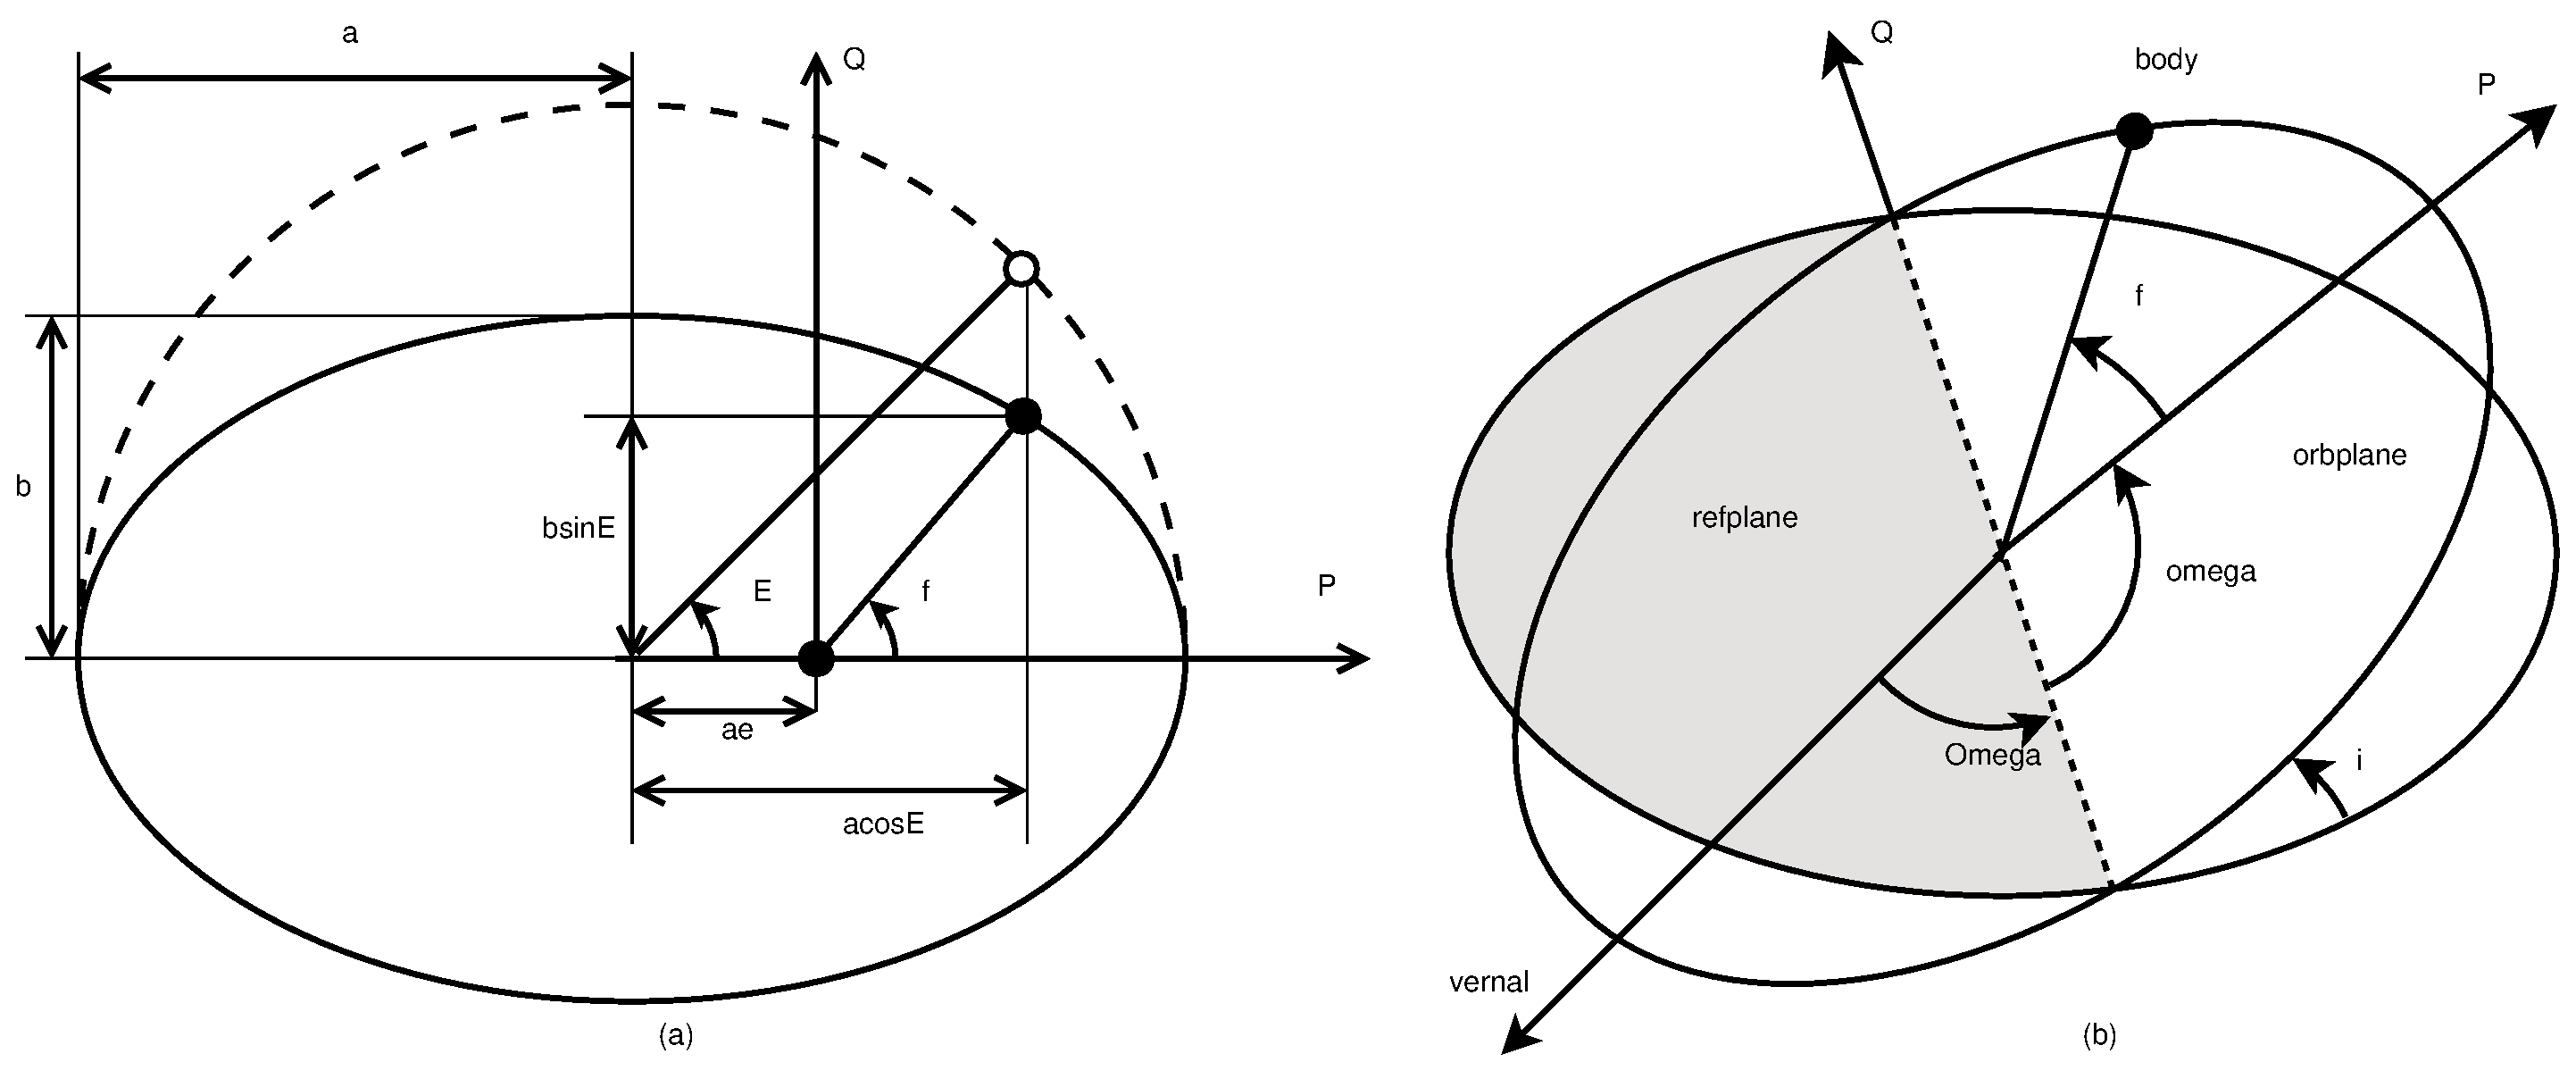
\includegraphics [angle=0, width=1.0\columnwidth] {figures/kepler.eps}
     \caption{\label{fig:perifocal}(a) Perifocal coordinates and the geometry of the 
     orbit. (b) Relation of the perifocal system to inertial systems.}
  \end {center}
\end {figure} 
\emph{Perifocal coordinate (PQW) system} has a origin at the focus of the orbit
and the axes are defined as follows:
\begin {itemize}
  \item The P axis points to the periapsis.
  \item The Q axis points to true anomaly of $90^\circ$.
  \item The W axis is orthogonal to the orbital plane.
\end {itemize}
In PQF frame, the position of a satellite can be written (see Figure \ref{fig:perifocal}):
\begin {eqnarray}
  \label{eq:PQF}
  \vc r_{PQF} 
  = 
  \begin {bmatrix}
    a\left(\cos E - e\right) \\ 
    b\sin E \\ 
    0
  \end {bmatrix}
  =
  |r|
  \begin {bmatrix}
    \cos f \\ 
    \sin f \\ 
    0
  \end {bmatrix}
  ,
\end {eqnarray}
where $a, b, e, E, f$ are the semi-major axis, semi-minor axis, eccentricity and 
eccentric anomaly, natural anomaly, respectively. 

To compute the velocities in the PQF frame, we first note that 
\begin {eqnarray}
  \diff{M^d}{t}
  =
  \diff{}{t}\left(
  E^d - \frac{180^\circ}{\pi}\,e\:\sin\frac{\pi E^d}{180^\circ}
  \right)
  = 
  \left(1 - e\:\cosd E^d\right)\diff{E^d}{t}.
\end {eqnarray}
Substituting orbital period, we obtain the \emph{mean angular motion}
\begin {eqnarray}
  n := \diff{M^d}{t} = \frac{360^\circ}{T} = \frac{180^\circ}{\pi}\sqrt{\frac{\mu}{a^3}}.
\end {eqnarray}
Substituting this back leads to 
\begin {eqnarray}
  \diff{E^d}{t} = \frac{n}{1 - e\:\cosd E^d}.
\end {eqnarray}
Thereafter, 
\begin {eqnarray}
  \vc v_{PQF} 
  =
  \diff{E^d}{t}
  \begin {bmatrix}
    -a\:\sind E^d \\
     \:\:\:b\:\cosd E^d \\
     0
  \end {bmatrix}
  =
  \diff{E^d}{t}
  \frac{\pi}{180^\circ}
  \begin {bmatrix}
    -a\:\sind E^d \\
     \:\:\:b\:\cosd E^d \\
     0
  \end {bmatrix}
  =
  \dfrac{\sqrt{\dfrac{\mu}{a^3}}}{1 - e\:\cosd E^d}
  \begin {bmatrix}
    -a\:\sind E^d \\
     \:\:\:b\:\cosd E^d \\
     0
  \end {bmatrix}.
\end {eqnarray}

\subsubsection{Computation of OSV from Elements}
The PQF coordinates are related to the frame of the orbital elements by 
rotations:
\begin {eqnarray}
  \label{eq:kepler_pos}
  \vc r &=& R_z(-\Omega)R_x(-i)R_z(-\omega) \vc r_{PQF}\\
  \label{eq:kepler_vel}
  \vc v &=& R_z(-\Omega)R_x(-i)R_z(-\omega) \vc v_{PQF}
\end {eqnarray}
where $\Omega, i, \omega$ are the longitude of ascending node, inclination 
and argument of periapsis, respectively. In $(\ref{eq:kepler_vel})$, it is 
assumed that the change in the orbital elements is slow enough not to affect 
velocity calculations.

\subsubsection{Solution of the Kepler Equation}
Suppose orbital elements $(a, e, i, \Omega, \omega, M)$ are known at 
specific time. The eccentric anomaly is solved from the \emph{Kepler Equation}:
\begin {eqnarray}
  \label{eq:kepler}
  M &=& E - e\sin E.
\end {eqnarray}
The equation $(\ref{eq:kepler})$ is expressed in radians. In degrees,
\begin {eqnarray}
\label{eq:kepler_deg}
M^d &=& E^d - \frac{180^\circ}{\pi}e\:\sind E^d.
\end {eqnarray}
This corresponds to a Newton-Raphson iteration
\begin {eqnarray}
  E^d_{n+1} &=& E^d_n 
  - 
  \frac{M_n^d - E_n^d + (180^\circ e/\pi)\:\sind{E_n^d}}{e\:\cosd(E_n^d) - 1}.
\end {eqnarray}
Thereafter, the position can be calculated using $(\ref{eq:PQF})$ and 
$(\ref{eq:kepler_pos})$.

\subsubsection{Computation of Osculating Elements}
Since every OSV corresponds to a unique Keplerian orbit, osculating elements 
can be solved from the OSV. The following discussion desribes how osculating
elements can be computed in (approximately) inertial coordinate system, where 
$\vu z$ is parallel to the specific angular momentum associated to the orbital 
plane.

For elliptic orbits, the semi-major axis can be written using the 
\emph{specific orbital energy} $E=v^2/2 - \mu/r$:
\begin {eqnarray}
  a = -\frac{\mu}{2E} 
  = \frac{\mu}{2}\left(\frac{1}{2}v^2 - \frac{\mu}{r}\right)^{-1}
  = \left(\frac{v^2}{\mu} - \frac{2}{r}\right)^{-1}.
\end {eqnarray}
The \emph{specific angular momentum} is defined as
\begin {eqnarray}
  \vc h &:=& \vc r\times\vc v.
\end {eqnarray}
The inclination is obtained 
\begin {eqnarray}
  i &=& \textrm{arccos}\frac{h_z}{|\vc h|}.
\end {eqnarray}
The eccentricity vector is obtained directly from the theory of Keplerian 
orbits
\begin {eqnarray}
  \vc e = \frac{1}{\mu}\left[
    \left(v^2 - \frac{\mu}{r}\right)\vc r - (\vc r\cdot\vc v)\vc v
  \right]
  = 
  \frac{\vc v\times\vu z}{\mu} - \frac{\vc r}{|\vc r|}.
\end {eqnarray}
The semi-minor axis can be now computed
\begin {eqnarray}
  b = a\sqrt{1 - e^2}.
\end {eqnarray}
The \emph{node vector} is defined as 
\begin {eqnarray}
  \vc n := \frac{\vu z\times\vc h}{|\vu z\times\vc h|}.
\end {eqnarray}
The node vector is orthogonal to both the orbital and the 
equatorial/ecliptic planes. It is parallel to the direction associated
to the ascending node. The intersection with the equatorial/ecliptic plane 
occurs at direction $\vu n = (\cos\Omega, \sin\Omega, 0)$. Thus, 
\begin {eqnarray}
  \Omega = \textrm{atan2}\left(n_y, n_x\right) 
  = 
  \textrm{atan2}\left(h_x, -h_y\right).
\end {eqnarray}
The eccentricity vector can be written
\begin {eqnarray}
  R_z(-\omega)R_x(-i)R_z(-\omega)
  \begin {bmatrix}
  a(1-e) \\ 0 \\ 0
  \end {bmatrix}
  = 
  a(1-e)
  \begin {bmatrix}
  \cos\Omega\cos\omega - \sin\Omega\cos i\sin\omega \\
  \sin\Omega\cos\omega + \cos\Omega\cos i\sin\omega \\
  \sin i\sin\omega 
  \end {bmatrix}
  =
  \begin {bmatrix}
  e_x \\
  e_y \\
  e_z
  \end {bmatrix}.
\end {eqnarray}
In case of $\sin i=0$, this reduces to 
\begin {eqnarray}
  \begin {bmatrix}
    \cos\Omega\cos\omega - \sin\Omega\sin\omega \\ 
    \sin\Omega\cos\omega + \cos\Omega\sin\omega \\ 
    0
  \end {bmatrix}
  =
  \begin {bmatrix}
    \cos(\Omega + \omega) \\
    \sin(\Omega + \omega) \\
    0
  \end {bmatrix}
  = 
  \begin {bmatrix}
    e_x/a \\ 
    e_y/a \\
    0
  \end {bmatrix}
\end {eqnarray}
This yields 
\begin {eqnarray}
  \omega = \textrm{atan}(e_y, e_x) - \Omega, \quad \textrm{when} \: \sin i = 0.
\end {eqnarray}
When $\sin i\neq 0$, we obtain 
\begin {eqnarray}
  \frac{e_z}{\sin i} = \sin\omega.
\end {eqnarray}
Also depending on the value of $\Omega$, we obtain the relations 
\begin {eqnarray}
  \frac{1}{\cos\Omega}\left(
    e_x + \frac{\sin\Omega\cos i}{\sin i}e_z 
  \right)
  &=& \cos\omega \\ 
  \frac{1}{\sin\Omega}\left(
    e_y - \frac{\cos\Omega\cos i}{\sin i}e_z
  \right)
  &=&  \cos\omega
\end {eqnarray}
and finally 
\begin {eqnarray}
  \omega = 
  \left\{
    \begin {array}{rr}
    \textrm{atan2}\left(\dfrac{e_z}{\sin i}, 
    \dfrac{1}{\cos\Omega}\left[e_x + \dfrac{\sin\Omega}{\tan i}e_z\right]
    \right), & \cos\Omega\neq 0 
    \\
    \textrm{atan2}\left(\dfrac{e_z}{\sin i}, 
    \dfrac{1}{\sin\Omega}\left[e_y - \dfrac{\cos\Omega}{\tan i}e_z\right]
    \right), & \sin\Omega\neq 0 
    \end {array}
  \right.
\end {eqnarray}
To obtain the eccentric anomaly, we note 
\begin {eqnarray}
  \begin {bmatrix}
    \xi \\ \eta \\ 0 
  \end {bmatrix}
  =
  \begin {bmatrix}
    a(\cos E - e) \\ b\sin E \\ 0
  \end {bmatrix}
  =
  R_z(\omega)R_x(i)R_z(\Omega)\vc r,
\end {eqnarray}
which allows us to solve 
\begin {eqnarray}
  E = \textrm{atan2}(\eta/b, \xi/a + e).
\end {eqnarray}
The mean anomaly then follows from the Kepler equation.
\subsection{Orbital Coordinate Systems}

\begin{thebibliography}{1}
  \bibitem{gnss}
  E. Suirana, J. Zoronoza, M. Hernandez-Pajares,
  ``GNSS Data Processing - Volume I: Fundamentals and Algorithms'',
  European Space Agency, 2013.
  \bibitem{aiaa_frames}
  J. Seago, D. Vallado,
  ``Coordinate Frames of The U.S. Space Object Catalogs'',
  AIAA Publication 2000-4025,
  Astrodynamics Specialist Conference, Denver CO, Aug. 2000.
\end{thebibliography}  
\end {document}
